\documentclass{beamer}

\usepackage{graphicx}
\usepackage{listings}
\usepackage{textpos}

\begin{document}

\beamertemplatenavigationsymbolsempty

\title{DSP}
\subtitle{Uses, Performance, Comparison to Traditional MCUs}
\author{Dinker Ambe\\
John Collins\\
Alec Ten Harmsel}

\addtobeamertemplate{frametitle}{}{%
    \begin{textblock*}{70mm}(.96\textwidth,-0.75cm)
        
\includegraphics[clip=true,width=0.20\textwidth]{m.png}
    \end{textblock*}
}

\frame{\titlepage}

\begin{frame}{Why Use a DSP?}
    \begin{itemize}
        \item Faster than a MPU, and more flexible than an FPGA
        \item Specific calculations used in processing analog signals are much faster with DSP
	\begin{itemize}
                \item Multiply Accumulate 
                \item Finite Impulse Response
                \item Compare
        \end{itemize}
        \item Only pipelined architecture won't cut it:
	\begin{itemize}
                \item DSPs have parallel memory units to fetch multiple data and instructions at the same time
                \item Single cycle operations to make pipelining faster
                \item Hardware controlled looping to minimize overhead
        \end{itemize}
        \item Multiple ALUs and computation units to perform instructions in parallel
        \item DSPs can perform well in a whole class of computation related to real-life signals in 'real time'
        \item For Example, Hexagon DSP by Qualcomm can exceute FFT loop in 1 clock cycle
	\begin{itemize}
                \item The same FFT loop implementation in a RISC architecture would take 29 instructions.
        \end{itemize}
    \end{itemize}
\end{frame}

\begin{frame}{History}
    \begin{itemize}
        \item Need for a solution that can execute complex math required for DSP
        \item Originally, DSP applications implemented using bit-slice processors
        \item First DSP created by TI in 1978, used in Speak \& Spell children's toy
        \item Second generation ~(80s) processors become standalone devices
        \item Third generation ~(90s) procesors allow hardware acceleration for complex math
        \item Fourth generation (current), higher clock speeds, smaller packaging, reduced price
    \end{itemize}
\end{frame}

\begin{frame}{What Is A DSP?}
    \begin{itemize}
        \item Specialized processor for Digital Signal Processing
        \item Capabilities of a DSP:
            \begin{itemize}
                \item Measure
                \item Filter
                \item Compare
            \end{itemize}
        \item These actions are perfomed on analog signals
        \item Most multiprocessors can perform these tasks
            \begin{itemize}
                \item But DSPs get better performance to power 
                \item Used in low-power, mobile, with a need for speed 
            \end{itemize}
     \end{itemize}
\end{frame}

\begin{frame}{What Is A DSP?}
    \begin{itemize}
        \item Requirement for low-latency
            \begin{itemize}
                \item Most DSP algorithms must be performed on a lot of incoming data
                \item Must be calculated repeatedly
                \item Used when there is a constrained time limit for calculations
                    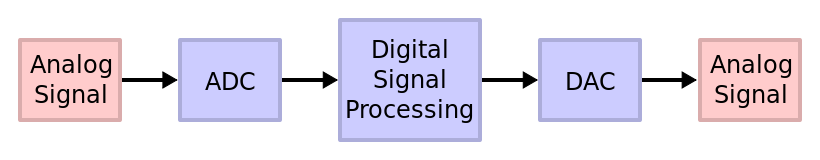
\includegraphics[width=0.6\textwidth]{block_diagram.png}
            \end{itemize}
        \item Can Perform Add, Sub, Mult, and Div very quickly and efficiently
	\item Wide range of power and performance (Texas Instruments)
	     \begin{itemize}
                \item Ultra-low power 16-bit with FFT acceleration (300 MHz)
                \item Power Optimized 32-bit fixed/float DSP (1+ GHz)
                \item High performance multicore 32-bit accellerated DSP (16 GHz)
            \end{itemize}
     \end{itemize}
\end{frame}

\begin{frame}{What Is A DSP?}
    \begin{itemize}
        \item Dedicated parallel multipliers
        \item Dedicated parallel ALUs
        \item Dedicated shifter
        \item DMA Memory Controller
        \item Dedicated FFT Hardware
        \item Example: Analog Devices' Blackfin Architecture
            \begin{itemize}
                \item 2x 16-bit MACs
                \item 2x 40-bit ALUs
                \item 4x 8-bit ALUs
                \item 1x 40-bit Shifter
            \end{itemize}
        \item Example: Texas Instruments' TMS320C55x Architecture
            \begin{itemize}
                \item 2x 16-bit MACs
                \item 1x 40-bit ALU
                \item 1x 16-bit ALU
            \end{itemize}
    \end{itemize}
\end{frame}

\begin{frame}{Uses}
    \begin{itemize}
        \item Real-time data transformation
            \begin{itemize}
                \item Cable box
                \item Audio receiver
                \item Sound cards
                \item Automotive sensing
                \item Network switching
            \end{itemize}
        \item High throughput, low power data transformation
            \begin{itemize}
                \item Audio/Video transcoding
                \item Cryptocurrency mining
            \end{itemize}
        \item Not for running a "modern" operating system % No virtual memory
        \item Not for generic workloads % Can't take advantage of hardware
    \end{itemize}
\end{frame}

\begin{frame}{ISA}
    \begin{itemize}
        \item Mostly math instructions
        \item Special instructions
            \begin{itemize}
                \item MAC (Multiply accumulate)
                \item FIR (FIR filter)
                \item Square Distance
            \end{itemize}
        \item Typically can have two (or more) opcodes in an instruction for
            math instructions
        \item Few features: small interrupt table, no MMU, etc.
    \end{itemize}
    % Blackfins only have 7 or 9 configurable interrupts
    % MPUs are common, but no MMU for virtual memory
    % Typically have kernel and user mode
    % Parallel MAC, parallel math and store, etc.
\end{frame}

% Plots only show fixed point, 16-bit MAC units. This is a litte biased, since
% everything high-performance from TI is floating point.
\begin{frame}{Performance vs. Price}
    \begin{center}
        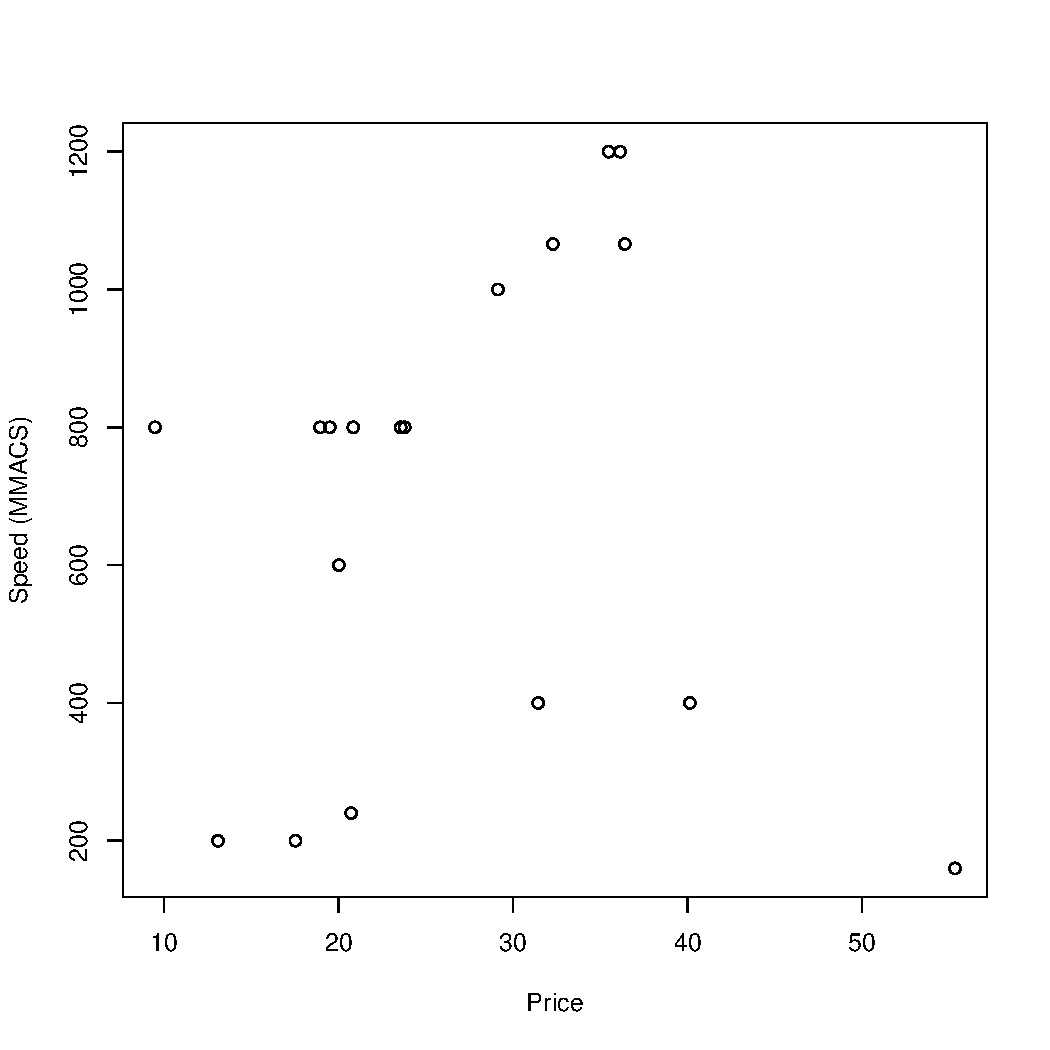
\includegraphics[width=0.8\textwidth]{price_perf.pdf}
    \end{center}
    % TI outlier is due to non-pipelined arch
    % Discuss pipelining and amortized single-cycle MACs
\end{frame}

\begin{frame}{Performance vs. Power}
    \begin{center}
        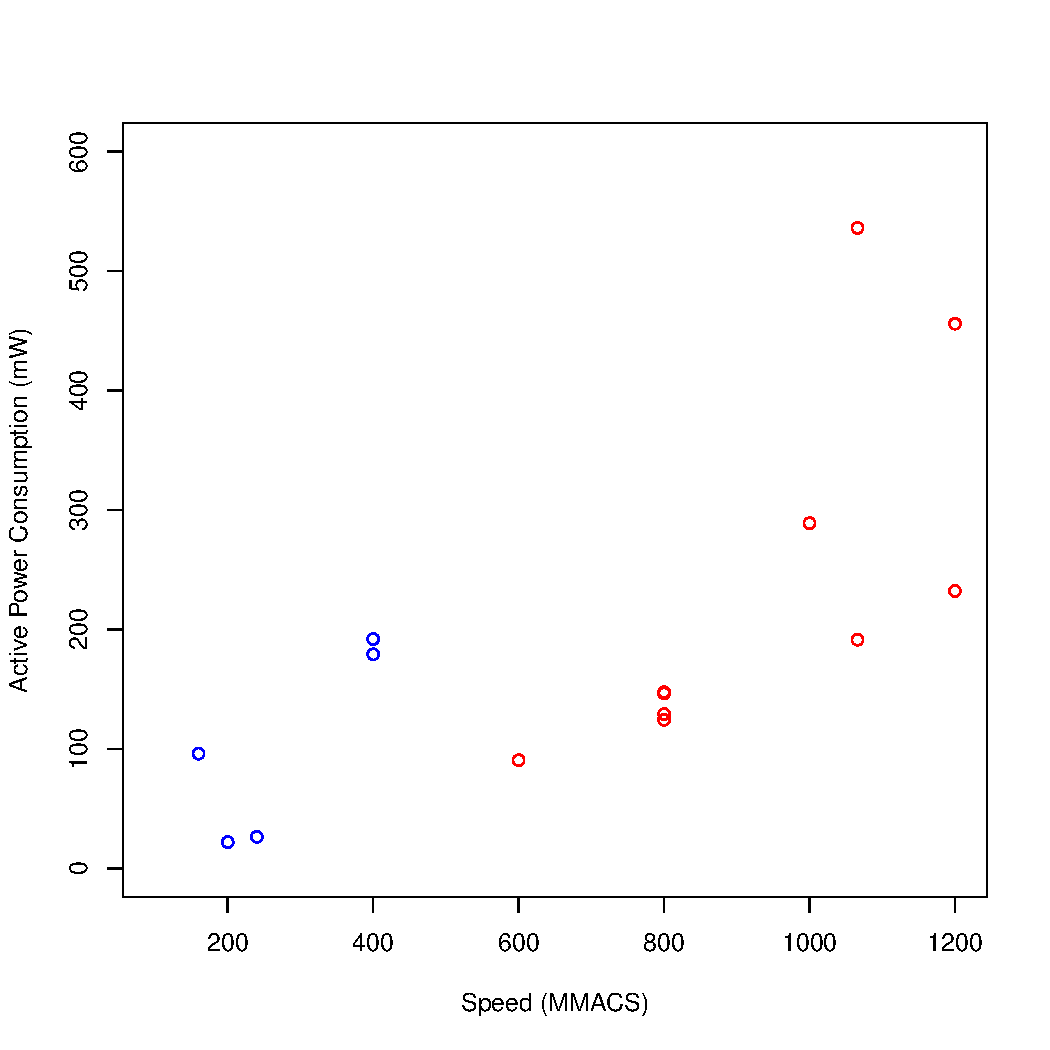
\includegraphics[width=0.8\textwidth]{power_perf.pdf}
    \end{center}
\end{frame}

\begin{frame}{How To Program a DSP}
    \begin{itemize}
        \item Architecture Description
            \begin{itemize}
                \item All available memory
                \item Memory mapped to external peripherals
            \end{itemize}
        \item Source Code Generation
            \begin{itemize}
                \item Slow but easy: High level languages such as C
                \item Fast but difficult: processor's native assembly
                \item Compromise: High level for generic functions, assembly for DSP computations
            \end{itemize}
    \end{itemize}
\end{frame}

\begin{frame}{FIR Filter in C}
    \begin{center}
        {\tiny
            \lstinputlisting{fir_example.c}
        }
    \end{center}
\end{frame}

\begin{frame}{FIR Filter in Assembly}
    \begin{center}
        {\tiny
            \lstinputlisting[firstline=52]{fir_example.s}
        }
    \end{center}
    % This is only the FIR part of the assembly. No interrupt setup or other
    % setup is shown.
\end{frame}

\begin{frame}{FIR in Assembly in a C program}
    \begin{center}
        {\tiny
            \lstinputlisting[firstline=36]{fir_asc_example.c}
        }
    \end{center}
\end{frame}

\end{document}
